\section{Historical Overview}
Over the past century, cosmological observations have profoundly reshaped our understanding of the universe. From observations of \citet{1925Obs....48..139H} measuring the distances to spiral nebulae, including the Andromeda Galaxy, it showed that these `nebulae' were actually galaxies outside the Milky Way. Later in \citet{1929ApJ....69..103H}, it was shown that galaxies are receding from us at velocities proportional to their distances, leading to the formulation of Hubble's Law, and the revolutionary concept of an expanding universe. Years later, the discovery of the cosmic microwave background (CMB) radiation by \citet{1965ApJ...142..419P} provided compelling evidence for the Big Bang theory, suggesting that the universe originated from a hot and dense state approximately 13.8 billion years ago. Subsequent satellite missions like the Cosmic Background Explorer (COBE; \citealt{1992ApJ...396L...1S}) and the Wilkinson Microwave Anisotropy Probe (WMAP; \citealt{2003ApJS..148...97B}) measured the CMB with unprecedented precision finding anisotropies of $\sim 10^{-6}$ K. In the 1970s, Rubin and Ford analyzed galaxy rotation curves and found that galaxies rotate at speeds that cannot be accounted for by the visible matter alone \citep{1970ApJ...159..379R, 1980ApJ...238..471R}. This discrepancy provided strong evidence for the existence of dark matter, a mysterious form of matter that does not emit, absorb, or reflect light. Dark matter is now understood to constitute about 26\% of the universe's mass-energy content, while Baryon, making up our visible world, constitutes only 5 \%. The late 1990s witnessed the surprising discovery that the expansion of the universe is accelerating, based on observations of distant Type Ia supernovae by the Supernova Cosmology Project and the High-Z Supernova Search Team \citep{1998AJ....116.1009R, 1999ApJ...517..565P}. This acceleration implies the existence of dark energy, an enigmatic force that permeates all of space and makes up approximately 68\% of the universe's total mass-energy budget. In 2015, the Laser Interferometer Gravitational-Wave Observatory (LIGO) made the first direct detection of gravitational waves providing direct evidence for the existence of gravitational waves, confirming a key prediction of General Relativity, opened a new window for observing cosmic events \citep{2016PhRvL.116f1102A}. As observational technologies continue to advance, ongoing and future discoveries promise to further refine our understanding of the universe, addressing the remaining mysteries of dark matter, dark energy, and the fundamental forces shaping the universe.

From a theoretical standpoint, the cornerstone of modern cosmology is 
Einstein's General Theory of Relativity, formulated in 1915 \citep{1915SPAW.......844E}. General Relativity provides the fundamental framework for explaining gravitational phenomena on cosmic scales, including the dynamics of the universe's expansion, black holes, and gravitational lensing effects. Building upon Einstein's equations, \citet{1922ZPhy...10..377F} and \citet{1931MNRAS..91..483L} independently derived solutions that describe a homogeneous and isotropic universe. These solutions led to the concept of an expanding or contracting universe and forms the mathematical foundation for the standard cosmological model. In the late 1940s, \citet{1948Natur.162..680G}, along with his collaborators \citet{1948Natur.162..774A}, proposed the Big Bang nucleosynthesis theory, which explains the formation of light elements like hydrogen and helium in the early universe. 
\citet{1968ApJ...153....1P}, \citet{1969Ap&SS...4..301Z} further developed the theory of the recombination era, when the universe cooled enough for electrons and protons to combine into neutral hydrogen, allowing photons to travel freely, creating the CMB radiation. Sequently, the theory of Baryonic Acoustic Oscillations (BAO) was introduced by \citet{1970Ap&SS...7....3S}, and independently by \citet{1970ApJ...162..815P}, which describes the imprint of primordial sound waves in the distribution of galaxies and the CMB. To address the Big-Bang's challenges, the concept of cosmic inflation was introduced by \citet{1981PhRvD..23..347G}, \citet{1982PhLB..108..389L}, and others. Together, these theories contribute to a comprehensive picture of the universe's origin, composition, and evolution.

\section{Astronomical Surveys and Observations}
Astronomical surveys are extensive observational projects designed to map large regions of the sky with high depth and precision, producing critical datasets for fundamental questions in astrophysics and cosmology. They aim to test the standard cosmological model ($\Lambda$CDM) by providing precise measurements that can confirm or challenge it, addressing issues like the Hubble tension—a discrepancy in expansion rate measurements from early~\citep{2016A&A...594A..13P} and late~\citep{2019ApJ...876...85R} observations—and inconsistencies in parameters such as $S_8$. Surveys also study the formation and evolution of cosmic structures by mapping millions of galaxies and dark matter distributions using techniques like cosmic shear and galaxy-galaxy lensing\citep{2013MNRAS.432.1544M, 2022PhRvD.105b3520A}.

\noindent These surveys employ different methodologies: 

Imaging surveys capture wide-field images across multiple wavelengths to map cosmic structures and analyze galaxy populations (e.g., HSC~\citep{2018PASJ...70S...4A}, SDSS~\citep{2019BAAS...51g.274K}, DES~\citep{2018ApJS..239...18A}, LSST~\citep{2019ApJ...873..111I}), while spectroscopic surveys collect spectral data revealing redshifts, compositions, and kinematics essential for studying galaxy dynamics and the universe's expansion (e.g., PFS~\citep{2016SPIE.9908E..1MT}, BOSS~\citep{2013AJ....145...10D}, DESI~\citep{2016arXiv161100036D}, KiDS with spectroscopic extensions~\citep{2013Msngr.154...44D}).

They can be ground-based, utilizing Earth-based telescopes but limited by atmospheric effects (e.g., HSC, DES, KiDS), or space-based, operating above Earth's atmosphere for higher clarity and sensitivity, especially in inaccessible wavelengths (e.g., HST~\citep{2001ApJ...553...47F}, the upcoming Nancy Grace Roman Space Telescope\citep{2015arXiv150303757S}, and the Euclid mission\citep{2010arXiv1001.0061R}).

Surveys are also classified into Stage-III and Stage-IV based on technological sophistication and scale~\citep{2006astro.ph..9591A}. Stage-III surveys (e.g., DES, KiDS, HSC) represent the current generation aiming to refine cosmological parameters and deepen understanding of dark energy and dark matter. Stage-IV surveys (e.g., Rubin Observatory~\citep{2019ApJ...873..111I}, DESI, the upcoming Roman Space Telescope) are the next generation characterized by scale and precision, aiming for high-precision cosmological measurements and deeper exploration of dark energy and dark matter.

Several significant galaxy surveys have been designed to measure weak lensing signals with high precision. Table~\ref{tab:survey_comparison} provides a comprehensive overview of four pivotal surveys focusing on their observational capabilities.
\begin{table}[h]
    \centering
    \caption{Comparison of Key Galaxy Surveys for Weak Lensing}
    \label{tab:survey_comparison}
    \begin{tabular}{lccc}
        \toprule
        \textbf{Survey} & \textbf{Area (deg$^2$)} & \textbf{Approx. Galaxy Density (arcmin$^{-2}$)} & \textbf{Median Redshift} \\
        \midrule
        DES/KiDS & $\sim$5,000 &  7 & 0.4 \\
        HSC Wide & $\sim$1,400 &  15 & 0.7 \\
        LSST & $\sim$18,000 & 30 & 1.0 \\
        \textit{Roman}/\textit{Euclid} & $\sim$2,000 & $50$ & 1.5 \\
        \bottomrule
    \end{tabular}
\end{table}

The Dark Energy Survey (DES; \citealt{2005astro.ph.10346T, 2018ApJS..239...18A, 2021ApJS..255...20A}) utilized the 570-megapixel Dark Energy Camera (DECam; \citealt{2015AJ....150..150F}) mounted on the 4-m Blanco Telescope at the Cerro Tololo Inter-American Observatory (CTIO) in Chile. Over the course of its operation, DES observed more than 300 million galaxies across approximately 5,000~deg$^2$ of the southern sky in five optical bands ($g$, $r$, $i$, $z$, $Y$). It achieved an effective galaxy density of about $\sim 6$~arcmin$^{-2}$ and provided photometric redshift estimates up to $z \sim 1.2$. The data collected by DES has made significant contributions to cosmology and astrophysics, including precise measurements of cosmic shear~\citep{2022PhRvD.105b3514A} and galaxy clustering~\citep{2022PhRvD.105b3520A}. 

The Hyper Suprime-Cam Subaru Strategic Program (HSC-SSP; \citealt{2018PASJ...70S...4A}) comprises three layers: Wide, Deep, and UltraDeep, conducted with the 8.2-m Subaru Telescope equipped with the 870-megapixel Subaru Hyper Suprime-Cam (HSC; \citealt{2018PASJ...70S...1M}). The Wide layer covers approximately 1,400~deg$^2$, yielding galaxy densities of around $\sim 15$~arcmin$^{-2}$. Photometric redshifts extend up to $z \sim 2$. The superior imaging quality of HSC enhances the accuracy of weak lensing measurements and contributes to tighter cosmological constraints \citep{2019PASJ...71...43H}. Currently, HSC is preparing its final data release (Y6) ending STAGE-III surveys.

The future Legacy Survey of Space and Time (LSST; \citealt{2009arXiv0912.0201L, 2019ApJ...873..111I}) is conducted at the Vera C. Rubin Observatory. Over a 10-year period, LSST will survey approximately 18,000~deg$^2$ of the sky. It is expected to detect around 20~billion galaxies, corresponding to galaxy densities exceeding $\sim 30$~arcmin$^{-2}$, with redshift measurements up to $z \sim 3$. LSST's vast dataset will substantially improve the statistical precision of weak lensing analyses and further refine cosmological models \citep{2012arXiv1211.0310L}.

Finally, the \textit{Nancy Grace Roman Space Telescope} (\emph{Roman}; \citealt{2015arXiv150303757S}) will conduct wide-field near-infrared imaging and spectroscopy from space scheduled for launch in the mid-2020s. Covering approximately 2,000~deg$^2$. The expected galaxy densities exceed $\sim 50$~arcmin$^{-2}$, facilitated by its space-based observations. The mission aims to provide spectroscopic redshifts higher than $z \sim 3$, significantly enhancing the precision of weak lensing measurements.

\section{Constraint from Weak Lensing}
While $\Lambda$CDM has been successful in explaining a wide range of cosmological observations, several tensions have emerged between different datasets. statistically significant discrepancy of about $4$ to $5\sigma$ between the value of the Hubble constant ($H_0$) inferred from the Planck CMB measurements \citep{2021CQGra..38o3001D} and the late-time measurements of local universe cosmic distance ladder measurements \citep{2022ApJ...934L...7R}. In addition to the Hubble tension, discrepancies have been observed in the measurements of the parameter $S_8 \equiv \sigma_8 \sqrt{\Omega_m/0.3}$, where $\sigma_8$ represents the root-mean-square amplitude fluctuation of matter density measured in spheres of $8\, h^{-1}\,\mathrm{Mpc}$, and $\Omega_m$ is the present-day matter density parameter. Several large-scale structure (LSS) experiments have reported $2$ to $3\sigma$ lower values of $S_8$ compared to those inferred from Planck CMB data \citep{2019PASJ...71...43H, 2021A&A...645A.104A, 2021JCAP...10..030G}.

Some of the strongest constraints on $S_8$ from LSS observations come from the study of cosmic shear, which is the weak gravitational lensing of distant galaxies by the intervening LSS along the line of sight. 
These small, coherent distortions in the shapes of background galaxies are sensitive to both the amplitude of matter density fluctuations ($\sigma_8$) and the growth of these fluctuations over cosmic time \citep{2001PhR...340..291B, 2010CQGra..27w3001B, 2015RPPh...78h6901K}. While there is a degeneracy between $\Omega_m$ and $\sigma_8$ in cosmic shear analyses, the product $S_8$ is tightly constrained \citep{2015RPPh...78h6901K, 2018ARA&A..56..393M}. Assuming a flat ΛCDM cosmological model and utilizing cosmic shear catalogs, recent analyses from major surveys have measured the cosmological parameter $S_8$: DES year 3 analysis reports $S_8 = 0.759^{+0.025}_{-0.023}$ \citep{2022PhRvD.105b3514A, PhysRevD.105.023515} using two-point correlation functions (2PCFs) and $S_8 = 0.793^{+0.038}_{-0.025}$ \citep{2022MNRAS.515.1942D} using power spectra ($C_\ell$s). The KiDS-1000 analysis reports $S_8 = 0.759^{+0.024}_{-0.021}$ \citep{2021A&A...645A.104A} using 2PCFs and $S_8 = 0.754^{+0.027}_{-0.029}$ \citep{2022A&A...665A..56L} using $C_\ell$s. The HSC year 3 analysis measure $S_8 = 0.769^{+0.031}_{-0.034}$ \citep{2023PhRvD.108l3518L} using 2PCFs and $S_8 = 0.776^{+0.032}_{-0.033}$ \citep{2023PhRvD.108l3519D} using $C_\ell$s.

As demonstrated in recent analyses, fully and robustly quantifying the cosmological constraints from cosmic shear necessitates accurate estimation and mitigation of various systematic sources and astrophysical effects, which are natural phenomena influencing observations \citep{2023PhRvD.108l3519D}. Imperfect modeling of the Point Spread Function (PSF), which characterizes the telescope's response to point sources, can introduce systematic errors in galaxy shape measurements \citep{2023MNRAS.525.2441Z}. Additionally, uncertainties in the redshift distribution, referring to errors in determining the distances to galaxies, can bias estimates of cosmological parameters \citep{2023MNRAS.518..709Z}. Shear calibration biases, which are systematic errors in measuring the distortion of galaxy shapes, encompass several specific issues: galaxy model bias resulting from incorrect models of galaxy shapes \citep{2010MNRAS.406.2793B}, noise bias introduced by measurement noise \citep{2012MNRAS.425.1951R}, selection bias arising from the preferential selection of certain types of galaxies \citep{2000ApJ...537..555K}, and detection bias caused by errors in the detection process \citep{2020ApJ...902..138S}. These biases significantly impact the measured cosmic shear signal and are typically calibrated using image simulations \citep{2018MNRAS.481.3170M}. Furthermore, baryonic feedback processes, which involve interactions from supernovae and active galactic nuclei \citep{2016MNRAS.459.1468M, 2018MNRAS.480.3962C}, and intrinsic alignments, referring to the non-random orientations of galaxies due to local gravitational fields \citep{2015SSRv..193....1J, 2015SSRv..193..139K, 2015SSRv..193...67K}, must be carefully controlled to avoid biased cosmological inferences.

\section{Higher-Order Statistics in Weak Lensing}
Traditionally, the power spectrum has been the primary statistical measure used to quantify the distribution of matter density fluctuations in the universe \citep{2019PASJ...71...43H, 2023PhRvD.108l3519D}. However, the weak lensing field is inherently non-Gaussian due to the nonlinear evolution of structures under gravity, leading to features resulting from gravitational collapse, mergers, and other astrophysical processes. The power spectrum, being a two-point statistic, captures only the Gaussian aspects of the field and thus cannot fully characterize these non-Gaussian features.

To fully leverage the information contained in the weak lensing field, it is essential to employ higher-order statistics that are sensitive to the non-Gaussianities. Various higher-order statistics have been studied in the past, such as: higher-order moments \citep{2015PhRvD..91j3511P, 2020MNRAS.498.4060G}, Minkowski functionals \citep{2019JCAP...06..019M, 2022OJAp....5E..13G, 2024arXiv241000401A}, probability distribution function \citep{2021MNRAS.505.2886B, 2023arXiv230405928T, 2023OJAp....6E...1U}, Peak and Minima Counts \citep{2018MNRAS.474..712M, 2024MNRAS.528.4513M}, three-point statistics \citep{2004MNRAS.348..897T, 2014MNRAS.441.2725F}, and deep learning \citep{2018JCAP...10..051F, 2022PhRvD.105h3518F}. Employing these higher-order statistics enhances the cosmological constraining power of weak lensing analyses, potentially alleviating tensions in parameter estimates and providing deeper insights into the underlying physics. 

Figure~\ref{fig:Euclid_Forecast} \citep{2023A&A...675A.120E} shows the forecasted constraints on the cosmological parameters $\Omega_m$ and $\sigma_8$ from the Euclid mission using ten different higher-order statistics. It is demonstrated that by combining any of these statistics with the standard two-point statistics, The constraints on $\Omega_m$ and $\sigma_8$ improve by a factor of $2$ to $3$ for individual parameters and by a factor of $4.5$ for their combination. This highlights the potential of higher-order statistics to probe non-Gaussian features in the weak lensing field and enhance the precision of cosmological parameter estimates.

\begin{figure}[ht]
    \centering
    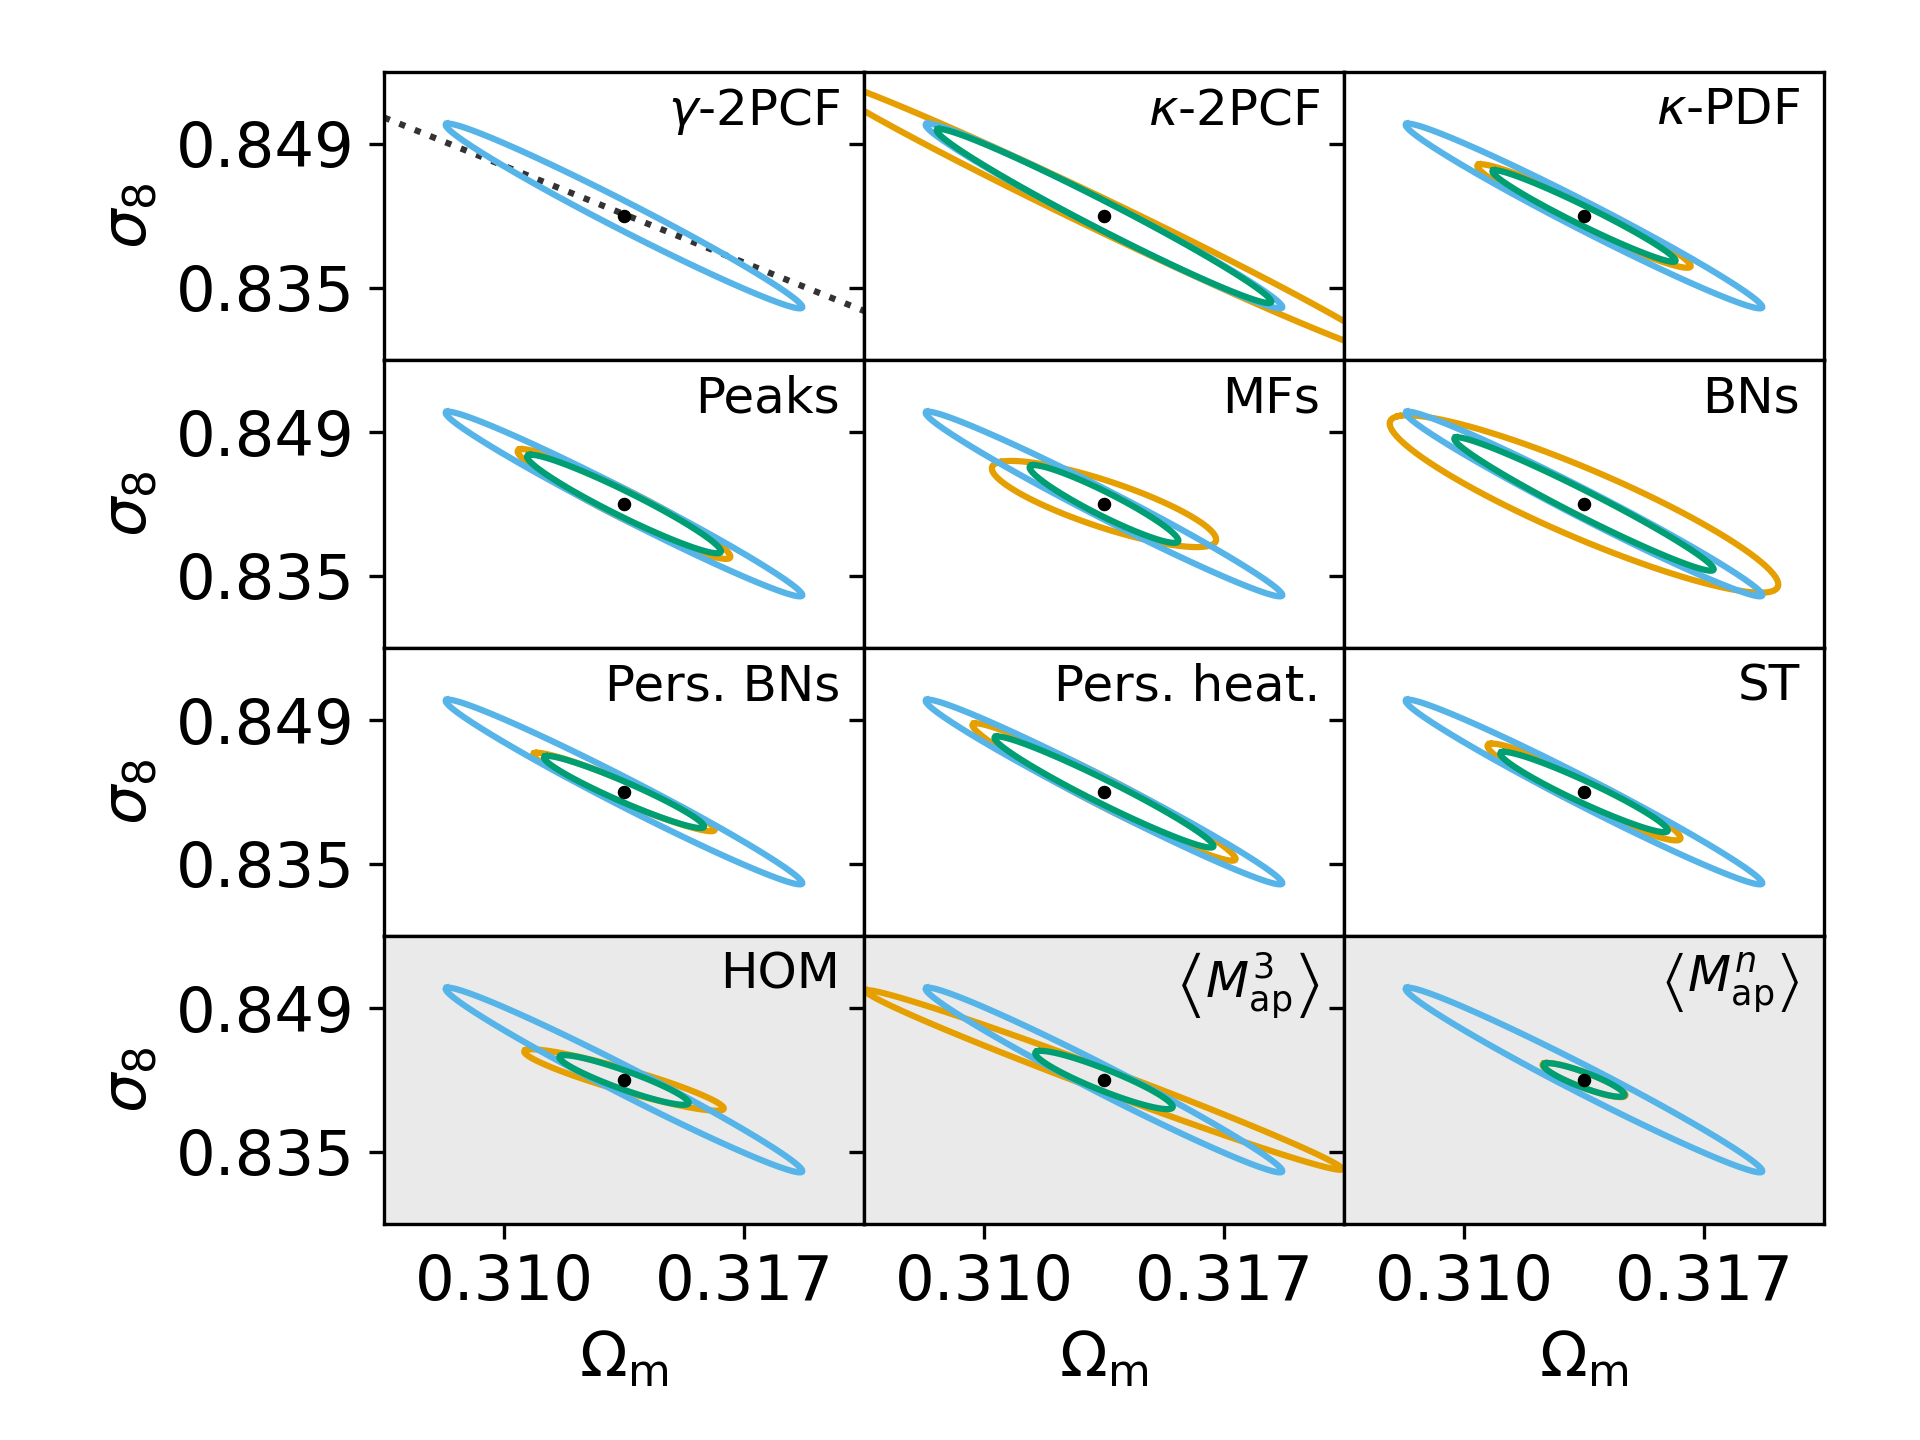
\includegraphics[width=\textwidth]{figures/Euclid_Forecast.png}
    \caption[Forecasted constraints on $\Omega_m$ and $\sigma_8$ from the Euclid mission using ten different higher-order statistics]{Forecasted constraints on $\Omega_m$ and $\sigma_8$ from the Euclid mission using ten different higher-order statistics. The figure demonstrates the potential improvements in parameter constraints achievable by incorporating higher-order statistics along with two-point statistics in weak lensing analyses. Figure adapted from \citet{2023A&A...675A.120E}}
    \label{fig:Euclid_Forecast}
\end{figure}

However, accurately estimating cosmological constraints from these higher-order statistics necessitates precise knowledge of the model uncertainties measured from the covariance matrices. The covariance matrix quantifies the uncertainties and correlations between different statistical measures and is crucial for techniques like Fisher forecasting and likelihood analyses that predict parameter constraints \citep{1997PhRvL..79.3806T}. To estimate these covariance matrices, we apply the same statistical measurements to a large ensemble of mock datasets that mimic real observations, accounting for the survey's specific characteristics, such as cosmic variance \citep{PhysRevLett.102.021302}, shot noise \citep{2019MNRAS.490.2606W} and super-sample covariance (SSC; \citealt{PhysRevD.87.123504}). SSC arises from the correlation between observed modes and modes whose wavelengths are larger than the survey size. For instance, if the observed region is embedded in a large-scale super-survey overdensity, the structures within the survey have evolved faster compared to a region embedded in the cosmic mean density. For weak lensing surveys, these mock datasets are generated through ray-tracing simulations of light propagation through the universe, using light cones constructed from cosmological N-body simulations \citep{2019MNRAS.486...52S, 2024arXiv240513495E}.

One common approach is to stack multiple multi-resolution simulation boxes to generate non-repeating lightcones that cover a wide range of redshifts \citep{2015MNRAS.448.2987F, 2015MNRAS.453.1513C, 2017ApJ...850...24T, 2019ApJ...875...69D}. While this method successfully captures the evolution of structures over cosmic time, it can struggle with achieving high redshift resolution and requires significant computational resources. Alternatively, repeating a single simulation box multiple times along the line of sight to construct the lightcone retains high redshift resolution and is computationally efficient \citep{2010ApJ...709..920S, 2018JCAP...03..049L, 2020JCAP...10..012S, 2024MNRAS.530.5030O}. However, this repetitive box method introduces artefacts like box replication effects \citep{2024MNRAS.534.1205C}. These effects can lead to underestimation of the variance on large scales and biases in the mean values of statistical measures, potentially impacting the estimation of cosmological parameters \citep{2021JCAP...01..028Z}.

\section{Aim of this Thesis}
The overarching goal of this thesis is to enhance the precision and reliability of cosmological constraints derived from higher-order weak lensing statistics by addressing key challenges in the estimation of their covariance matrices. Specifically, we focus on the impact of super-sample covariance (SSC) and box replication effects in simulations used for weak lensing analyses.

While super-sample covariance has been extensively studied and is well-understood for the power spectrum \citep{PhysRevD.87.123504, 2017JCAP...11..051B, 2018JCAP...06..015B}, its influence on higher-order statistics remains largely unexplored. Existing theoretical predictions for covariances that include SSC effects \citep{2023A&A...672A.185L, 2023OJAp....6E...1U} have not yet been thoroughly tested for these higher-order statistic \citep{2023A&A...675A.120E}. Moreover, while the impact of SSC has been studied in three-dimensional (3D) box simulations \citep{PhysRevD.108.043521}, its effects in two-dimensional (2D) weak lensing simulations have not been systematically examined.

Our first aim is to fill this gap by investigating how SSC affects higher-order weak lensing statistics and their covariance matrices. To achieve this, we conduct two sets of simulations:
\begin{description}
    \item[\textbf{BigBox Simulations}] --- Large-volume simulations that naturally include super-survey modes, capturing the SSC effects inherent in the Universe's large-scale structure.
    \item[\textbf{Tiled Simulations}] --- Simulations that replicate smaller boxes to cover the desired light cone, which will suppress super-survey modes and thus underestimate SSC.
\end{description}
By comparing the results from these two simulation strategies, we assess the extent to which SSC impacts the estimation of cosmological parameters using higher-order statistics. We examine how the covariance matrices are affected by varying smoothing scales and shape noise levels, which are crucial properties in weak lensing analyses. This comprehensive study allows us to determine the reliability of cosmological parameter estimations and to identify the conditions under which SSC effects become significant.

The second aim of this thesis is to investigate the impact of box replication effects in weak lensing simulations. As introduced earlier, the box replication is a common technique used to extend the effective simulation volume by periodically replicating a single simulation box along different axes. While this method is computationally efficient and retains high redshift resolution, it introduces artificial periodicity and can lead to under-predicts the variance of the imulations on large scales \citep{2021JCAP...01..028Z}.

Previous studies have examined box replication effects primarily for power spectrum and other statistical moments, focusing on biases in mean values \citep{2024MNRAS.534.1205C}. Also, \citet{2019PhRvD.100f3514F} studied the impact of the replication scheme on the predictions of the power spectrum and Convolutional Neural Networks (CNN) by increasing the boxsize and number of particles in a reference simulation while keeping the particle density constant. 
However, the impact on higher-order statistics and their covariance matrices has not been thoroughly explored. Considering that higher-order statistics are more and more used in weak lensing analyses, it is essential to understand how box replication affects these statistics and their covariance matrices. By investigating these effects, we aim to provide guidelines for future surveys to mitigate these artefacts and improve the accuracy of their cosmological parameter estimates.

By addressing these two key challenges, this thesis contributes to the broader effort of maximizing the scientific return of weak lensing surveys. Accurate covariance estimation is essential for improving the precision of cosmological parameter constraints derived from higher-order statistics, enhancing the utility of these statistics for probing the underlying physics of structure formation and dark matter, and guiding the design of future survey experiments.

\section{Structure of the Thesis}
This thesis dissertation is organized into nine chapters that systematically develop the theoretical framework, methodologies, and empirical analyses pertinent to the research objectives outlined in the previous sections.

In Chapter~\ref{chap:cosmology}, we provide a comprehensive overview of modern cosmology, tracing the historical development of the field and highlighting key theoretical milestones that have shaped our current understanding of the universe. 

Chapter~\ref{chap:weak_lensing} focuses on the theoretical basic concepts and observational aspects of weak gravitational lensing. 

In Chapter~\ref{chap:statistics}, we explore the summary statistics employed in weak lensing analyses to extract cosmological information from observational data, focusing on the power spectrum and higher-order statistics. 

Chapter~\ref{chap:covariance} addresses the theoretical prediction of covariance matrices including super-sample covariance and how the covariance affects the cosmological constraints. 

In Chapter~\ref{chap:simulation}, we review the numerical methods in astrophysics and cosmology, focusing on the N-body simulations and weak lensing simulations. 

In Chapter~\ref{chap:methods}, we introduce the methodologies used in this thesis, including the simulation strategies, data generation, statistical measurements, and covariance matrix estimation.

In Chapter~\ref{chap:results}, we present the results of our analyses, comparing the mean values and covariance matrices of higher-order statistics derived from the BigBox and Tiled simulations, examining how SSC influences the variances and correlations in the data.

The thesis concludes with Chapter~\ref{chap:conclusions}, where we summarize the key contributions and conclusions of this research. We reflect on how the work advances our understanding of super-sample covariance and box replication effects in the context of higher-order weak lensing statistics.